\documentclass{article}
\usepackage{color}
\usepackage{float}
\usepackage{floatflt}
\usepackage{graphicx}
\usepackage{hyperref}
\usepackage[utf8]{inputenc}
\usepackage{listings}
\usepackage{units}

\newcommand\Nch{$N_{ch}$}
\newcommand\dNdEta{$dN_{ch}/d\eta$}

\definecolor{mygray}{gray}{0.5}

\lstset{language=C++,
        numbers=left,
        numberstyle=\color{mygray}\scriptsize,
        showstringspaces=false,
        breaklines=true,
        basicstyle=\ttfamily\small,
        keywordstyle=\color{blue}\ttfamily,
        stringstyle=\color{magenta}\ttfamily,
        commentstyle=\color{green}\ttfamily}

\begin{document}

\tableofcontents
\newpage


\section{Introduction}
The charged-particle multiplicity measurement is a basic but very important analysis when studying the properties of heavy ion collisions and hence the forming quark gluon plasma (QGP). On a very basic level, the number of charged particles leaving the interaction region is counted. This measurement can be used to deduce properties of the QGP such as the energy density. This analysis follows two papers, which were performed in the past on different LHC datasets.
\begin{enumerate}
\item \label{itm:paper1} \href{http://arxiv.org/abs/1004.3034}{Charged-particle multiplicity measurement in proton-proton collisions at $\sqrt{s} = $ \unit[0.9] and \unit[2.36]{TeV} with ALICE at LHC}
\item \label{itm:paper2} \href{http://cds.cern.ch/record/1562873}{Charged-particle multiplicity measurement with Reconstructed Tracks in pp Collisions at $\sqrt{s} = $ \unit[0.9] and \unit[7]{TeV} with ALICE at the LHC}
\end{enumerate}
Additional information and detailed explanations of the physical background can be found in the following PhD Thesis:
\begin{enumerate}
\setcounter{enumi}{2}
\item \label{itm:thesis} \href{http://cds.cern.ch/record/1175646/}{Measurement of the Charged-Particle Multiplicity in Proton-Proton Collisions with the ALICE Detector}
\end{enumerate}


\section{Background behind the analysis}

\subsection{Physical Quantities}
As mentioned above, counting the charged particles is the main task of this analysis. This number is called charged-particles multiplicity and is denoted by \Nch. Because of the relativistic equivalence of mass and energy $E=m c^2$,
\begin{floatingfigure}[r]{60mm}
\centering
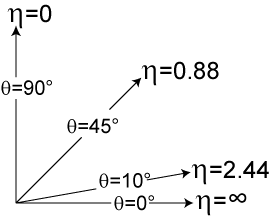
\includegraphics[width=40mm, natwidth=270, natheight=220]{images/Pseudorapidity.png}
\caption{Illustration of the pseudorapidity $\eta$ for a horizontal beamline; figure from \href{https://en.wikipedia.org/wiki/Pseudorapidity}{Wikipedia}}
\label{fig:eta}
\end{floatingfigure}
\noindent \Nch~ is directly related to the energy distribution inside the QGP. The multiplicity is mostly studied as density with respect to the pseudorapidity $\eta = \ln(\tan(\frac{\theta}{2}))$, which is a pure geometric quantity as figure \ref{fig:eta} illustrates. The resulting quantity is called multiplicity density \dNdEta~ and represents the amount of particles in an certain $\eta$ interval. In general, \dNdEta~ can depend on $\eta$ but in the following, the dependence is omitted in the notation.\\

\subsection{Normalization of \dNdEta}
The multiplicity density can rely on different normalizations, which means, different types of events are considered in the measurement.
The three types of inelastic collisions are \textit{non-diffractive (ND)}, \textit{single-diffractive (SD)} and \textit{double-diffractive (DD)}. Suggestively this corresponds to number of diffractive systems, which are created in the collision. A diffractive system is an excited incident particle, which carries the quantum numbers of the incoming particle. Figure \ref{fig:diff} illustrates the phenomenological difference between the different types of events. The two most used normalizations are \textit{total inelastic (INEL)} and \textit{non-single-diffractive (NSD)}. The first one contains all inelastic events (ND, SD and DD) while the second one contains only symmetric events (ND and DD). For further information see [\ref{itm:thesis}].
\begin{figure}
\centering
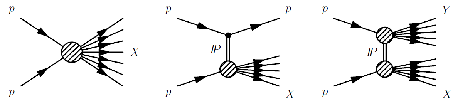
\includegraphics[width=\textwidth, natwidth=459, natheight=103]{images/diff.png}
\caption{From left to right: ND, SD and DD; figure from \href{www.inspirehep.net}{InspireHEP}}
\label{fig:diff}
\end{figure}

\subsection{The ALICE detector}
\href{http://aliceinfo.cern.ch/}{ALICE} (A Large Ion Collider Experiment), one of the four large experiments at the CERN Large Hadron Collider, has been designed to study heavy-ion collisions. It also studies proton-proton (pp) collisions, which primarily provide reference data for the heavy ion collisions. In addition, the pp-collision data allow for a number of genuine proton-proton physics studies.\\
The ALICE detector has been designed to cope with the highest particle multiplicities anticipated for collisions of lead nuclei at the extreme energies of the LHC. It is composed out of different sub-detectors. In the Central Barrel this are 
the \href{http://alipub.web.cern.ch/content/inner-tracking-system}{Inner Tracking System (ITS)}, consisting out of three detectors having each 2 layers, namely the Silicon Pixel Detector (SPD), the Silicon Strips Detector (SSD) and the Silicon Drift Detector (SDD). The two endcaps of the ITS contain 
the \href{http://alipub.web.cern.ch/content/v0-detector}{VZERO} trigger system. The ITS is followed radially by
the \href{http://alipub.web.cern.ch/content/time-projection-chamber}{Time Projection Chamber (TPC)}, 
the \href{http://alipub.web.cern.ch/content/transition-radiation-detector}{Transition Radiation Detector (TRD)}, 
the \href{http://alipub.web.cern.ch/content/time-flight}{Time Of Flight detector (TOF)}, 
the \href{http://alipub.web.cern.ch/content/high-momentum-particle-identification-detector}{High Momentum Particle Identification Detector (HMPID)}, the two electromagnetic calorimeters 
EMCAL and 
\href{http://alipub.web.cern.ch/content/photon-spectrometer}{PHOS} as well as 
\href{http://alipub.web.cern.ch/content/alice-cosmic-ray-detector}{ACORDE}, the dedicated cosmic ray detector. In the following analysis the ITS as well as the TPC can be used. The TPC only covers the region $|\eta|<0.8 \Leftrightarrow |\theta|>48^{\circ}$, so the analysis is focused mainly on this region.

\subsection{The ALICE trigger system}
In run 1 of the LHC, the spacing between two bunches was \unit[50]{ns} with a peak luminosity of the order of \unit[$10^{33}$]{$cm^{-2} s^{-1}$}. This led to large amounts of data, generated by the detectors, which had to be processed. As not all produced data is relevant for certain physics studies,  LHC experiments have several detectors capable to act as fast trigger systems, sometimes in a correlated manner, and allowing to record mainly interesting data. For ALICE, the so called Minimum Bias trigger (MB) relies on an signal either in one of the VZEROs or in one detector of the ITS. 

\section{The \dNdEta~ analysis}

\subsection{How to run the analysis}
In order to run the analysis, it is recommended to use the masterclass GUI. Select the tab \textit{dNdEta Analysis}, chose one of the datasets with a desired number of files and click on the picture. All necessary data files will be downloaded and their paths are collected inside four text files: \textit{files.txt, filesPerugia0.txt, filesPerugia2011.txt and filesPhojet.txt}, one for the data and three for the Monte Carlos respectively. In order to run the analysis manually, just execute the \href{https://root.cern.ch/}{Root} macro \textit{dNdEta.C} by the following line, if the mentioned text files are present:
\begin{lstlisting}[numbers=none, language=bash]
aliroot dNdEta.C
\end{lstlisting}
A detailed explanation of the workflow is given in \ref{subsec:analysis} and \ref{subsec:correction}. The main settings of the analysis can be changed as described below. When the analysis in finished, two windows open. One contains the main result, the comparison of the data with predictions, the other is a Root browser, in which all relevant files and therefore all plots are loaded. For further details see \ref{subsec:results} and \ref{subsec:intermediate}.
\subsubsection*{Analysis mode}
The analysis mode determines, which detector parts shall be used. By default this is TPC and ITS. The active parts can be chosen by comment in/out the lines $41-42$ in \textit{run.C}:
\lstinputlisting[linerange={41-42}]{../../Masterclass/dNdEta/run.C}
\subsubsection*{Trigger mode}
The trigger mode, which is used for the analysis, can be chosen in \textit{run.C} in lines $47-48$:
\lstinputlisting[linerange={47-48}]{../../Masterclass/dNdEta/run.C}
\subsubsection*{Normalization}
The normalization can be chosen in \textit{correct.C} by commenting in/out one of the block in lines $34-90$, e.g. for INEL:
\lstinputlisting[linerange={45-50}]{../../Masterclass/dNdEta/correct.C}
\subsubsection*{Low $p_{T}$ cutoff}
The low transverse momentum cutoff is also defined in \textit{correct.C}. It is the second argument, when calling \textit{Finish} in the uncommented block, e.g. here it is set to $0.15$:
\lstinputlisting[linerange={48-48}]{../../Masterclass/dNdEta/correct.C}

\subsection{AliRoot}
The \dNdEta~ analysis is using the \href{http://aliweb.cern.ch/Offline/AliRoot/Manual.html}{AliRoot} framework, which contains the software libraries allowing to to perform detector simulation, reconstruction and physics analysis for the ALICE collaboration. The main workflow is event based and modular. This means each physics interaction event is processed separately and can be looped through several tasks. This leads to a very convenient way of plugging an analysis together while reducing the amount source code as well as its complexity. The single tasks are contained in one of the two main parts of the AliRoot framework, AliCore and AliPhysics. The first one contains basic tasks, e.g. for event processing or simulations, while the latter one contains mainly tasks for physical analysis. The tasks are chained together in a so called train model using a Root macro. The configuration to be defined by the user contains a set of environment variables, input and output data containers as well as the connection between the different analysis tasks.\\

\subsection{Workflow of the analysis}
As described in the previous section, the analysis is split into several tasks and steering macros. The top-level macro \textit{dNdEta.C} controls the main workflow, which looks as follows:
\begin{enumerate}
\item Run the analysis on simulated Monte Carlo data
\item Run the analysis on real data
\item Correct raw results with MC
\item Plot the final results as well as intermediate steps
\end{enumerate}
The first step is to predict the expected results by using Monte Carlo simulations. For this analysis, there are three different MC datasets available, the first one is \textit{Pythia} with tune \textit{Perugia0}, the second one is the same with rune \textit{Perugia2011} while the third one is \textit{Phojet}. Both datasets are processed with the macro \textit{run.C}, which is explained in detail below:
\lstinputlisting[linerange={13-13,22-22,31-31}]{../../Masterclass/dNdEta/dNdEta.C}
For each of this runs, the result is both, a prediction of what will be measured (\textit{analysis\_mc.root}) based on the MC truth, as well as a correction map (\textit{correction\_map.root}), which can be used to correct the measured data with respect to detector effects like geometry or efficiency. After each run, the results are saved in separate folders (\textit{perugia0}. \textit{perugia2011} and \textit{phojet}).\\
Afterwards, the measured data from the ALICE detector is analyzed. This is done with the same script as for the MC, but the details differ a little bit, see below:
\lstinputlisting[linerange={31-31}]{../../Masterclass/dNdEta/dNdEta.C}
Of course, there is no correction map created in this run. Furthermore, the results are raw and are not corrected for the mentioned detector effects (\textit{analysis\_esd\_raw.root}).\\
This correction are applied in the third step of the analysis. There are three different correction maps for each of the different MC generators. Thus, the raw data is corrected three times, once for each generator (lines 50, 59 and 68). The results (\textit{analysis\_esd.root}) are saved in the folders of the MC.\\
The last step of the analysis and the second half of the macro \textit{dNdEta.C} (l. 56 ff) contains the plotting of intermediate steps and the final result of the analysis, which is a comparison between the MC prediction and the measured data. This is the key to determine, if the underlying models of the MC and therefore the understanding of the QGP is correct or if the models have to be modified are replaced. Nevertheless, the intermediate plots are as important as the final result because they deliver information about the correctness of the analysis as well as the quality of the measurement.

\subsection{The data analysis}
\label{subsec:analysis}
Following the workflow of the \dNdEta~ analysis, \textit{run.C} is the first macro, which directly uses AliRoot on the data. As described above, the macro is used for analyzing the MC as well as the measured data. It can be used in two different modes, one for MC and one for data.\\
In the first case, one wants to run the analysis task itself as well as the correction task. This is done by setting the first argument $runWhat = 2$. Furthermore one indicates, that the data contains MC information by calling the macro with $requiredData = 1$. The third argument is a text file, which contains paths to the data files. The last argument is optional and can contain some additional settings for the tasks (for further information see \href{aliroot-docs.web.cern.ch/aliroot-docs/PWGUD_SELECTORS_DNDETA_Index.html}{AliRoot}). Thus, the calls for the MC are as seen above. For the data analysis, the macro call is slightly different. One only wants to do the analysis, not the correction task, so $runWhat = 0$. Furthermore, the required data is raw data $requiredData = 2$. The text file is modified respectively.\\
The first lines of the macro (l. $22-33$) are setting the basic structure of the analysis.
\lstinputlisting[linerange={22-33}]{../../Masterclass/dNdEta/run.C}
This contains technical features like defining include paths, as well as the initialization of the analysis manager, which contains all tasks and settings. Afterwards, a handler is defined, which forces the analysis to run on the local machine. Further details can be found at the end of the macro, where the functionality is explained in the comments:
\lstinputlisting[linerange={165-179}]{../../Masterclass/dNdEta/run.C}
The last three lines of this paragraph contain the definition of the input file handler. Especially line $32$ is important, because there the unused parts of the detector deactivated for the analysis.\\
Lines $35-53$ are one of the most important part of the analysis. Firstly, it is defined, which parts of the detector shall be used. For this analysis, either only the ESD is used or the whole ITS together with the TPC. By default, both systems are used. In order to use only the SPD, one has to comment line $41$ in and $42$ out:
\begin{lstlisting}[firstnumber=41]
  AliPWG0Helper::AnalysisMode analysisMode = AliPWG0Helper::kSPD | AliPWG0Helper::kFieldOn;
  // AliPWG0Helper::AnalysisMode analysisMode = AliPWG0Helper::kTPCITS | AliPWG0Helper::kFieldOn;
\end{lstlisting}
The second important option is the offline trigger. This is an additional trigger to the minimum bias trigger, which is applied online during data taking. There are two options available:
\begin{description}
\item[kAcceptAll]{No further trigger is applied to the data}
\item[kOneParticle]{At least one particle in the SPD is required}
\end{description}
As seen above, on has to comment in the desired setting, e.g. to accept all particles:
\lstinputlisting[linerange={47-48}]{../../Masterclass/dNdEta/run.C}
The last definition of the variable \textit{diffTreatement} is more technical and is used for the MC analysis.\\
Lines $55-73$ contain another important setting of the analysis, the track cuts.
\lstinputlisting[linerange={59-73}]{../../Masterclass/dNdEta/run.C}
These cuts are important to ensure a certain quality for the tracks of particles, which are used in the analysis. For the default analysis with TPC and ITS, the ALICE standard cuts from 2010 are used. For SPD only, no cuts are required. For further information look into \textit{CreateStandardCuts.C} or at \href{https://twiki.cern.ch/twiki/bin/view/ALICE/SelectionOfPrimaryTracksForPpDataAnalysis}{ALICE Track Selection}.\\
Lines $75-78$ are adding the first task to the analysis, the physical event selection. Afterwards, lines $80-135$ are adding the main tasks of the analysis. This depends on the given data and is controlled by the given value of $runWhat$, see above. Both definitions are similar, so only one will be explained in detail:
\lstinputlisting[linerange={84-108}]{../../Masterclass/dNdEta/run.C}
Firstly, the task is defined. Lines $88-97$ are applying the previously defined options, such as the trigger, to the task. Afterwards, lines $99-107$ add the task to the manager, set output filename and connect in- and output.\\
In the next two sections, some final settings are set. Lines $137-144$ are used only for MC runs while lines $146-154$ are loading the magnetic field from \textit{OCDB.root} file, which is the Offline Condition DataBase.\\
\lstinputlisting[linerange={146-154}]{../../Masterclass/dNdEta/run.C}
Finally, the analysis can be started:
\lstinputlisting[linerange={156-161}]{../../Masterclass/dNdEta/run.C}

\subsection{The correction task}
\label{subsec:correction}
After MC and data are analyzed, the correction task must be performed. For that, three files must be in the same folder:
\begin{itemize}
\item \textit{analysis\_mc.root}
\item \textit{correction\_map.root}
\item \textit{analysis\_esd\_raw.root}
\end{itemize}
The correction task is also controlled by a macro, \textit{correct.C}, which takes the above mentioned files as standard input parameters. The core algorithm is \textit{AlidNdEtaCorrection}, which is intantiated and configured in lines $4-10$:
\lstinputlisting[linerange={4-10}]{../../Masterclass/dNdEta/correct.C}

% Here, the background part must be put in. Don't forget to edit the source code quote in line 171

After defining the background, the correction can be done. The correction can be done for different normalizations (see above) and the different trigger sets. As an example, the INEL correction is explained in detail, the others can be commented out as needed:
\lstinputlisting[linerange={46-52}]{../../Masterclass/dNdEta/correct.C}
Firstly, an analysis object is created with a suggestive naming. The third line is the call of the function \textit{Finish}, which then performs the correction. Its arguments are as follows:
\begin{enumerate}
\item The correction object
\item The pT cut which has to be used
\item The kind of correction, which has to be performed
\item A naming tag for the correction
\item The number of background events
\end{enumerate}
Afterwards, the histograms after the correction are saved into the output file, which is by default \textit{analysis\_esd.root}. As mentioned above, the correction is done with all MC datasets. Hence, there are three potentially different corrected versions of the data available. These fluctuations are studied in context of systematic errors and can reach up to $4.1\%$ in total, which is used here. If the amount of used MC files is small, these fluctuations can be much larger. Nevertheless, in the rest of the analysis, an arithmetic average of both corrections is used as single result.

\subsection{Results...}
\label{subsec:results}
\begin{floatingfigure}[r]{55mm}
\centering
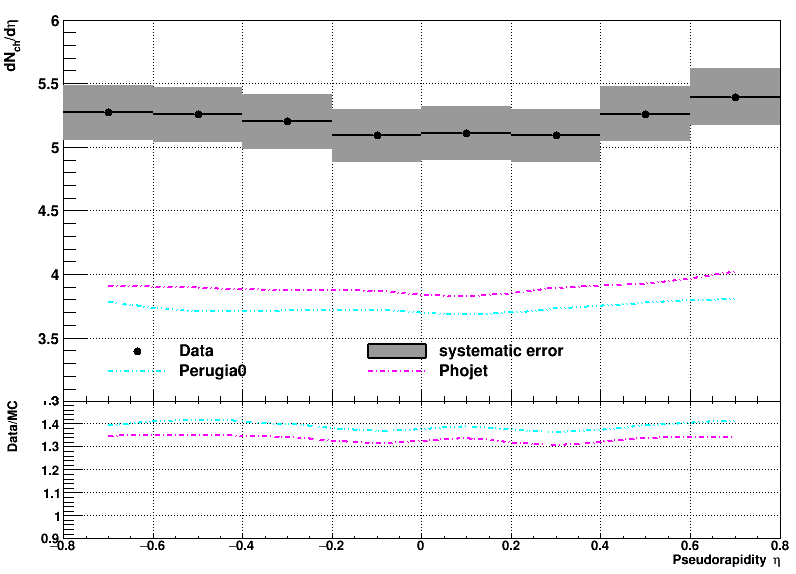
\includegraphics[width=45mm, natwidth=796, natheight=574]{images/dNdEta.png}
\caption{Example results of the \dNdEta~ analysis}
\label{fig:result}
\end{floatingfigure}
After the correction is done, the analysis is finished. The macro \textit{dNdEta.C} produces now a summary and comparison plot between the MC and the data. Such a plot can look like \ref{fig:result}. The plot is divided into two parts. The upper part shows the analyzed data as black points with error bars and with a gray error band. The error bars are due to statistical fluctuations. In figure \ref{fig:result}, the errors on \dNdEta~ are too small to be visible while the error on $\eta$ is due to the binning of the data. The gray band represents the mentioned systematic errors. As mentioned above, the amount of used MC files has a large influence on the correction. If only a few files are used, the visible error band is too small and does not represent the correct error estimation. Additionally to the data, the predictions of the three MC generators are plotted in the same diagram as colored lines. Their statistical errors are omitted here for simplicity but can be estimated by the change of the curvature and the asymmetry around $\eta = 0$. The lower plots show explicitly the difference between MC and data as a data/MC ratio. For accurate MC, this would be a straight line at 1.\\

\subsection{...and intermediate steps}
\label{subsec:intermediate}
Besides the final results, intermediate steps are interesting to control the single steps of the analysis as well as their quality. First of all, every plot is available in the concerning Root-files, which are produced during the analysis. After the analysis is finished, a Root browser is opened, in which the Root-files are already loaded. They can be found in the file tree on the left side in the folder \textit{ROOT Files}, which is the third from above. In the following part, some interesting intermediate plots are discussed. The headers represent the file and the path to the plot inside, followed by a description of it.
\subsubsection*{data/analysis\_esd\_raw.root/dndeta\_check\_vertex}
\begin{floatingfigure}[r]{50mm}
\centering
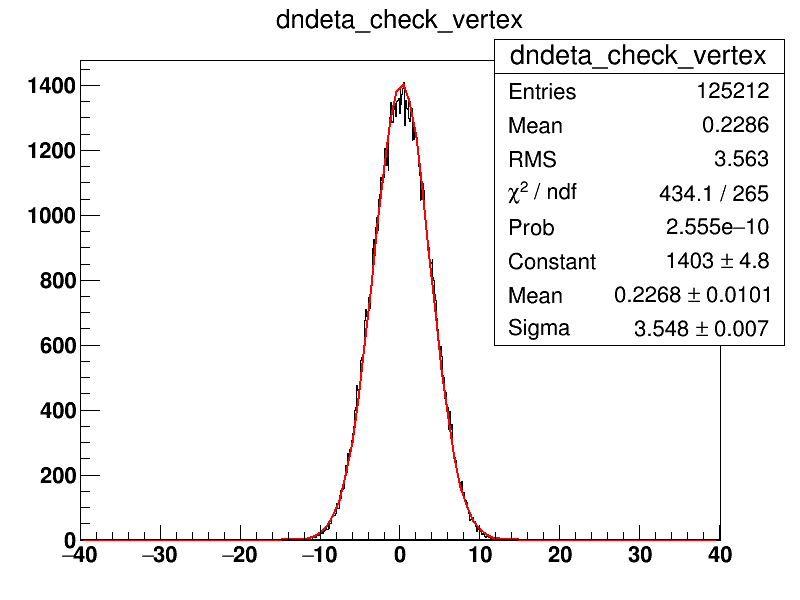
\includegraphics[width=50mm]{images/dndeta_vertex_check.png}
\end{floatingfigure}
\noindent The plots contains the reconstructed vertex positions of all events along the beam line axis in \unit{cm}. This is an important criteria to check the quality of the reconstruction. The distribution should follow a Gaussian with $\mu \approx 0$. This can be tested by fitting such a distribution. In order to do so, right-click on the black curve of the histogram, click \textit{Fit}, type \textit{gaus} into the field \textit{formula} and press OK. The width of the distribution is $\sigma \approx \unit[3.5]{cm}$ and the mean is $\mu < \unit[0.3]{cm}$. This is an intrinsic property of the beam at the interactions point of ALICE.\\
\subsubsection*{data/analysis\_esd\_raw.root/fMult(Vtx)}
The two plots show the multiplicity distribution in the raw data. The first one (fMult) contains all events while the latter one (fMultVtx) contains only those events, which have a reconstructed vertex. Normalized to $1$, this is equal to the multiplicity probability density $P(N_{ch})$, which is analyzed in the same paper as \dNdEta~ and contains information about how probable a certain multiplicity is. This density is another basic property to study the QGP.
\subsubsection*{data/analysis\_esd\_raw.root/dndeta\_check\_0}
This is the raw distribution of \dNdEta. It is not corrected for any detector effects and can contains asymmetries and other effects. This distribution has to be corrected by using the MC generators, which simulates the whole detector response.
\subsubsection*{data/analysis\_esd\_raw.root/fPhi}
The plots shows the distribution of reconstructed tracks in $\phi$-direction, which is the plane orthogonal to the beam line. In general, physics must be the same in $\phi$, the experiment is symmetric around the beam axis. Thus, a flat distribution is expected. In reality, fluctuations or even dips can be observed because the detector is not perfectly symmetric or even some parts of the detector can be damaged or offline.
\begin{figure}[H]
\begin{minipage}[b]{0.55\textwidth}
\subsubsection*{data/analysis\_esd\_raw.root/fRawPt}
This histogram contains the distribution of the transverse momentum of produced particles $\unit[p_{T}]{[GeV/c]}$. It can be useful to estimate a low-$p_{T}$-cutoff, which is used in the analysis.
\subsubsection*{*/analysis\_mc.root/dndeta\_check\_pt}
This is the same as above but for the MC dataset, which is chosen in the path (\textit{perugia0}, \textit{perugia2011} or \textit{phojet}). The combination of this with the distribution above can be used to estimate a low-$p_{T}$-cutoff, which has to be applied to the data. This cutoff is important because the ALICE detector is not sensitive to low $p_{T}$ particles and a cutoff therefore improves the quality of the analysis. The default value is $p_{T} > \unit[0.15]{GeV/c}$ above which the distributions are compatible.\\
\end{minipage}
\begin{minipage}[b]{0.45\textwidth}
\centering
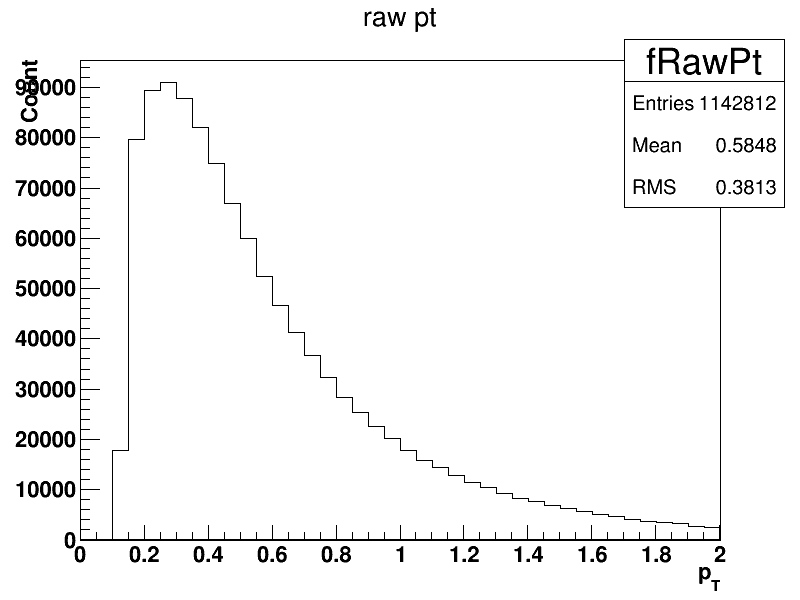
\includegraphics[width=\textwidth]{images/fRawPt.png}
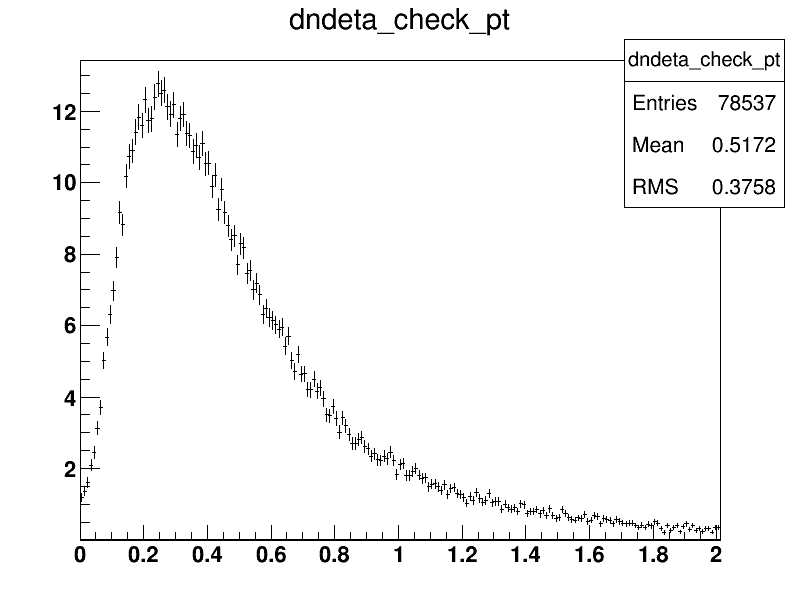
\includegraphics[width=\textwidth]{images/dndeta_check_pt.png}
\vspace{\baselineskip}
\end{minipage}
\end{figure}
\subsubsection*{*/analysis\_mc.root/dndeta*/dNdEta}
The plot shows the observed \dNdEta~ distributions of the MC simulations. The first * in the path stand again for the MC tool, while the second * indicates a special normalization/selection. The distribution is in general symmetric around $\eta = 0$ within its statistical uncertainty.
\subsubsection*{*/correction\_map.root/fEtaCorrelation}
This 2D-histogram show the correlation between the generated $\eta$ (x-axis) and the simulated measurement of $\eta$ in the detector (y-axis). This distribution should be as close and as sharp as possible to a line through the origin in order to make a precise measurement.
\subsubsection*{*/correction\_map.root/fEtaResolution}
Another form of representation of the above distribution is given in this plot. It is an histogram of the difference between generated $\eta$ and its simulated measurement. For a perfect detector, this would be a infinite sharp peak at exactly $0$, but in reality this is always smeared out.
\subsubsection*{*/correction\_map.root/fpT*}
In analogy to the two plots above, the generated and the simulated measurement of $p_{T}$ can be compared with the plots \textit{fpTCorrelation} and \textit{fpTResolution}. The first one is again a 2D-histogram while the second one represents the relative deviation (y-axis) in dependence of the generated $p_{T}$ (x-axis). This distribution should also be as narrow as possible to $0$.
\subsubsection*{*/analysis\_esd.root/dndeta*/dNdEta\_corrected}
This is the final result of the analysis with one specific MC. The second * in the path represents again one specific normalization/selection. This histogram is used in order to calculate the average of the different MC and also to estimate the systematic uncertainty coming from the MC. The latter one can be estimated by comparing this plot for the different available MC generators.
\subsubsection*{*/analysis\_esd.root/dndeta*/Pt}
The final distribution of transverse momenta can be obtained in this histogram. In contrast to the raw histograms of $p_{T}$, there are no entries below the cutoff, which has been applied during the analysis.


\end{document}
